\chapter{Aspects techniques}

	\section{Représentation d'un livre}

		\subsection{Représentation des noeuds}
			Il y a quatre type de noeud représenté par des classe (Voir \ref{BookNode}): \textbf{BookNodeWithChoices}, \textbf{BookNodeWithRandomChoices}, \textbf{BookNodeCombat} et \textbf{BookNodeTerminal}. Tous extends direct ou indirectement de \textbf{AbstractBookNode}. Cette dernière contient juste un texte pour le constructeur car toutes les méthodes contiennent au moins un texte.\\
			Pour l'ensemble des méthode représentant les différents type de noeuds, sauf le \textbf{BookNodeTerminal}, chacune d'entre elles contiennent des choix et une perte/gain de vie. Pour cela, ces dernières extends de la classe \textbf{AbstractBookNodeWithChoice} permettant ainsi de définir des variable tel que le nombre d'item à prendre, la liste des items disponible sur ce noeuds, la liste des items à acheter, un boolean qui oblige l'utilisateur à manger pour continuer, le nombre de vie perdu/gagner sur ce noeud, la liste de choix disponible. Ce dernier est défini par une List<T> car cela peut être un \textbf{BookNodeLink} ou un \textbf{BookNodeLinkRandom}. Ce qui veut dire que ça peut être soit un lien normal, soit un lien venant d'un noeud aléatoire.\\

			Pour le \textbf{BookNodeWithRandomChoices}, une méthode, en plus de son constructeur à été ajouté. En effet, elle permet de donner un choix random en fonction du nombre aléatoire généré ainsi que le nombre de chance de chaque lien. Cela ajoute d'abord tout les liens disponibles, c'est à dire, tout les liens où le joueur peut avoir accès en fonction des prérequis demandés, dans une liste nommé listNodeLinkDisponible. Si aucun lien n'est disponible, cela retourne null. Dans le cas contraite\ref{getRandomChoices}, cela choisi un nombre aléatoire en fonction de la somme total de chance de tout les liens valide.\\
			Puis, en fonction de ce nombre, la chance de chaque lien valide est enlever du nombre random jusqu'à ce que ce nombre soit égal ou inférieur à zéro. Le choix de la destination est alors retourné.\\
			\begin{lstlisting}[language=java, label=getRandomChoices]
				int nbrChoice = 0;
				Random random = new Random();
				int nbrRandomChoice = random.nextInt(somme);
				for (int i = 0 ; i < listNodeLinkDisponible.size() ; i++){
					if(!this.getChoices().get(i).isAvailable(state)){
						continue;
					}
					nbrRandomChoice -= this.getChoices().get(i).getChance();
					if(nbrRandomChoice < 0){
						nbrChoice = i;
						break;
					}
				}
				return this.getChoices().get(nbrChoice) ;
			\end{lstlisting}

			Pour le \textbf{BookNodeTerminal}, il prend en compte, en plus du texte de \textbf{AbstractBookNode}, un BookNodeStatus défini soit sur \textbf{FAILURE} soit sur \textbf{VICTORY}.

			\begin{figure}[H]
				\centering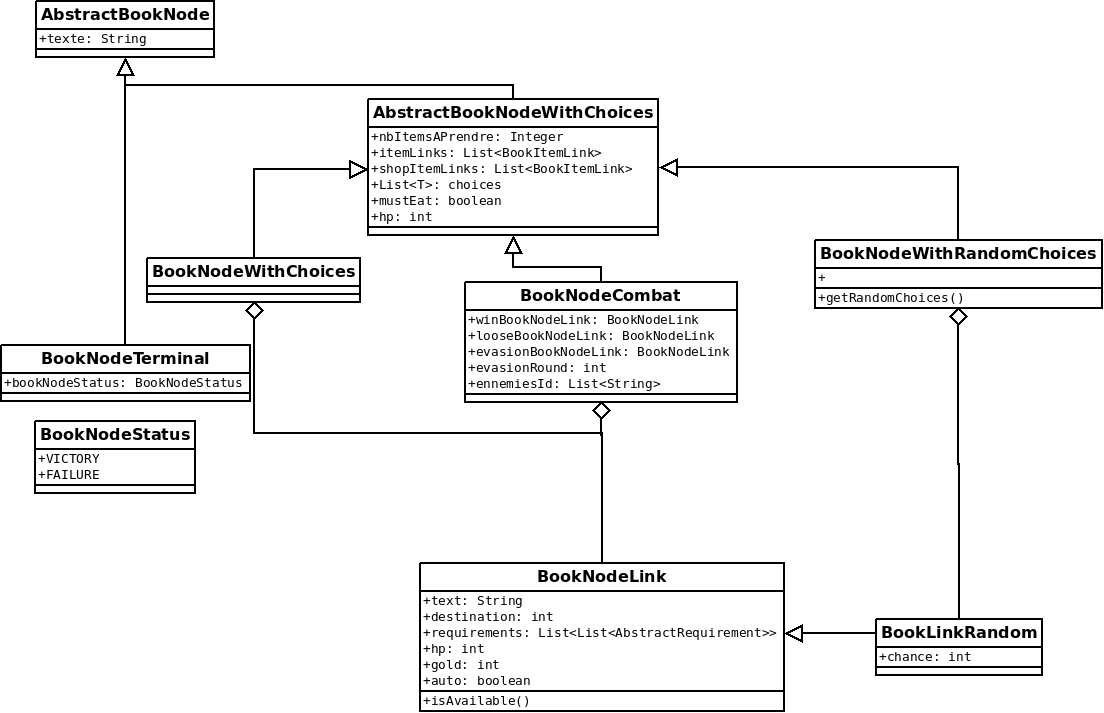
\includegraphics[width=0.70\textwidth]{img/BookNode.png}
				\caption{BookNode}
				\label{fig:BookNode}
			\end{figure}

		\subsection{Représentation des liens}
			Les noeuds sont lié par des liens. C'est liens sont soit défini par la classe \textbf{BookNodeLink} ou \textbf{BookNodeLinkRandom}. Pour évité les redondances, cette dernière extends de \textbf{BookNodeLink}. Elles prennent donc toutes les deux un texte, une destination (défini par le numéro du noeud) et enfin, une liste de prérequis.  Pour la destination, nous avons d'abord mis un AbstractBookNode, mais des instanceof était requis pour chaque appel de la destination. Nous avons alors choisis de changer et de mettre le numéro du choix correspondant.\\
			Pour le \textbf{BookNodeLinkRandom}, la classe à besoin d'une variable chance, afin de définir la chance d'aller vers ce noeud. Cette chance est ensuite totalisé sur tout les noeuds disponible, comme vu précédament\ref{getRandomChoices}.\\
			La classe \textbf{BookNodeLink} est composé d'une méthode, nommé isAvailable() permettant de savoir si le personnage principal à les items requis (défini par une liste de List<AbstractRequirement>) pour aller vers ce lien. S'il n'y a pas d'item requis, le player peut alors aller vers ce lien. Sinon, un appel de la fonction isSatisfied()\ref{isSatisfied}, vu un peu plus loin, sera utilisé afin de savoir si le personnage à chaque item/skill/money demandé. Si le player satisfait tout les prérequis demandé, cela retourne true. False dans le cas contraire.\\
			\begin{lstlisting}[language=java, caption=exemple de isAvailable(), label=isAvailable]
				for(List<AbstractRequirement> groupRequirement : requirements) {
					boolean satisfied = true;
					for(AbstractRequirement r : groupRequirement) {
							if(!r.isSatisfied(state)) {
								satisfied = false;
								break;
							}
						}

					if(satisfied)
						return true;
				}
				\end{lstlisting}



		\subsection{Prérequis pour un choix}
			Les prérequis des liens sont définir par une classe AbstractRequirement puis une classe par type de requirements. Il y a la classe \textbf{RequirementItem}, \textbf{RequirementMoney} ainsi que \textbf{RequirementSkill}. Tous extends de AbstractRequirement afin de pouvoir utiliser la méthode isSatisfied(), prenant en paramètre un BookState. Tous prennet un id en compte, permettant de retrouvé l'item/skill/money demandé. Car chaque type possède un id différent afin de pouvoir retrouvé l'objet/la compétence correspondant. La seul chose qui diffère c'est la quantité de money requis.\\
			Pour savoir si un item/skill est présent dans l'iventaire du presonnage principal, un for est utilisé afin de regarder les item/skill possédé. Si l'ID de l'item/skill n'est pas possédé, le personnage principal ne peut donc satisfaire tout les prérequis. Pour l'argent, une simple ligne permet de savoir, en fonction de l'ID de la money, savoir si le player en possède suffisament. Actuellement, une seule money est disponible, se nommant "gold". En effet, nous n'avons pas eu le temps de créer une boite de dialog ainsi qu'un espace dédié pour la création de différentes money.
			\begin{lstlisting}[language=java, caption=exemple de isSatisfied(), label=isSatisfied]
			public boolean isSatisfied(BookState state) {
				for (String i : state.getMainCharacter().getItems()){
					if(i.equals(itemId)) {
						return true;
					}
				}

				return false;
			}
			\end{lstlisting}


		\subsection{Représentation des personnages, items}

			Nous allons maintenant parler des personnages et des items du livre. Bien qu'il n'y ai pas grand chose à expliquer sur eux, car il s'agit de classes possédant beaucoup de getter et setter, nous souhaitons détailler certains choix faits.

			Commençons par les personnages. Ceux ci sont définits par la classe BookCharacter dans le package magic\_book.core.game. Cette classe possède presque uniquement des getter et setter bien qu'elle possède également quelques méthodes utilitaires.

			\begin{figure}[H]
				\centering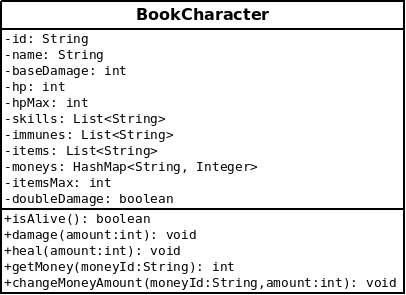
\includegraphics[width=0.45\textwidth, keepaspectratio]{img/book_character.png}
				\caption{UML sur la gestion des personnages}
			\end{figure}

			Concernant les listes de String (skills, immunes, items), il s'agit d'une liste contenant les id. Pour "immunes", il s'agit des id des skills contre lesquels le personnage est immunisé. Cela nous permet aux items et compétences de n'être référencés qu'à un seul et même endroit, c'est à dire, dans la classe Book. Pour la monnaie, le choix a été fait d'utiliser une HashMap<String, Integer> afin de pouvoir gérer différents types de monnaie et leur montant dans une même histoire. Malheureusement, notre format de livre, et donc notre application, ne permet pour le moment pas de gérer pleinement cette fonctionnalité.

			Passons maintenant aux items. Ceux-ci possèdent une classe mère BookItem dans le package magic\_book.core.item.

			\begin{figure}[H]
				\centering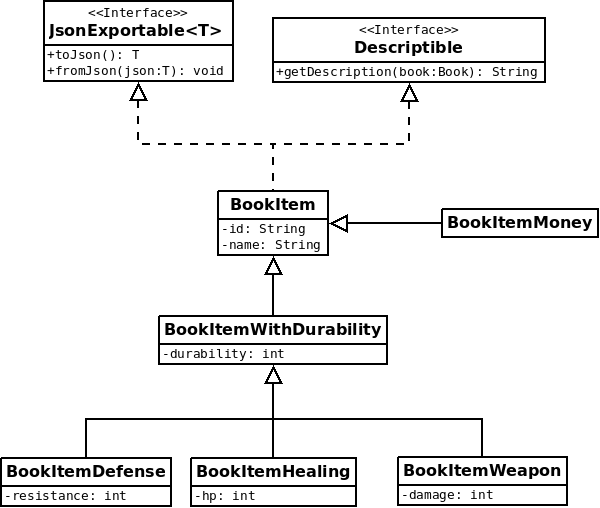
\includegraphics[width=0.66\textwidth, keepaspectratio]{img/book_item.png}
				\caption{UML sur la gestion des items}
			\end{figure}

			Avant de détailler notre choix, nous allons expliquer brièvement les deux interfaces que l'on observe. L'une se nomme Descriptible et permet à l'item de se décrire sous forme de String. Bien que la méthode \textit{String toString()} soit déjà prévu à cet effet, celle ci ne permet pas de prendre en argument un livre (classe Book). Bien entendu, c'est logique mais certains objets ont besoin du livre pour se décrire, par exemple, pour retrouver un item / personnage à partir de son id. La seconde interface, JsonExportable sera expliqué plus en détails dans \nameref{subsec:lecture_ecriture_fichier} à la page \pageref{subsec:lecture_ecriture_fichier}. Pour rester bref, disons qu'elle permet, la lecture et l'écriture du fichier en JSON.

			Dès lors, l'héritage prend son sens et permet une spécialisation d'un item de deux façons. La première, qui est la plus logique, permet l'ajout d'attribut spécfique à notre classe fille. Par exemple, il serait étrange d'avoir un attribut pour savoir combien de dégat un item de type money inflige. Deuxièmement, cette spécialisation intervient dans la redéfinition, par les classes filles, des méthodes des deux interfaces. En effet, chaque classe fille apporte ses propres attributs à chacune des différentes méthodes comme on peut le voir sur le listing ci-dessous. On nottera l'appel à la méthode définit dans la classe mère par le mot clé \textit{super.nomMethode(arguments)}.

			\begin{lstlisting}[gobble=12, language=Java, caption=Exemple de spécialisation des items]
			@Override
			public String getDescription(Book book) {
				StringBuffer buffer = new StringBuffer();

				buffer.append(super.getDescription(book));

				buffer.append("Dégats : ");
				buffer.append(damage);
				buffer.append("\n");

				return buffer.toString();
			}

			@Override
			public ItemJson toJson() {
				ItemJson itemJson = super.toJson();

				itemJson.setDamage(damage);
				itemJson.setItemType(ItemType.WEAPON);

				return itemJson;
			}
			\end{lstlisting}

		\subsection{La classe Book}

			Cette classe est la plus importante de tout le projet. En effet, c'est elle qui met en lien tous les différents éléments qu'on a pu évoquer avant. C'est en effet ce que l'on peut observer sur la figure suivante.

			\begin{figure}[H]
				\centering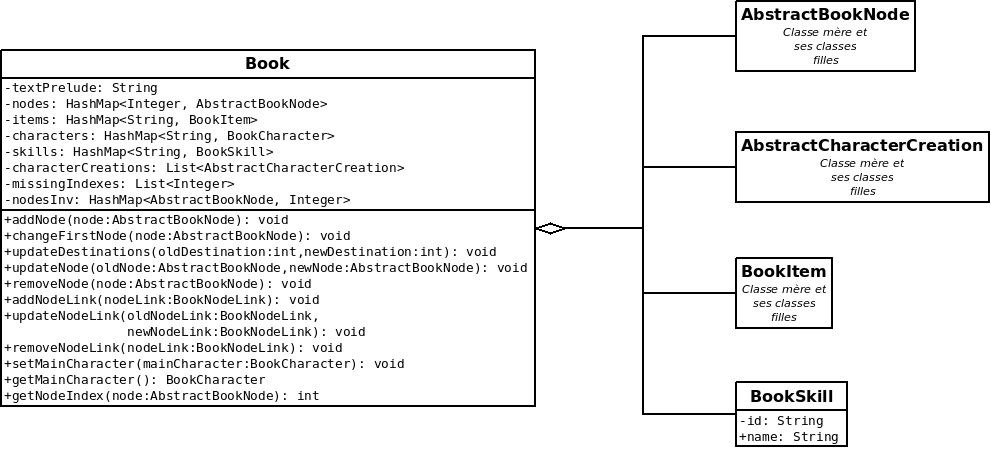
\includegraphics[width=0.8\textwidth, keepaspectratio]{img/book.png}
				\caption{UML sur la classe Book}
			\end{figure}

			Par soucis de place, les getters et setter n'ont pas été renseignés. Il en va de même pour le détails des différentes classes (BookCharacter, BookItem, ...). Enfin, les observateur sont volontairement omis car ils seront détaillés un peu plus tard (dans \nameref{subsec:pattern_observer} à la page \pageref{subsec:pattern_observer}).

			Tout d'abord, commençons par expliquer comment sont sauvegardés nos noeuds et les liens dans la HashMap "nodes".

			Cette HashMap possède un int comme clé, clé qui correspond au numéro du paragraphe. Lorsque l'on ajoute un noeud au livre, on doit d'abord lui trouver un numéro. Nous avons décidé de plusieurs règles. Les paragraphes commencent à partir du numéro 1. Le numéro 1 représente \textbf{toujours} le premier paragraphe du livre. De ce fait, si l'on ajoute un noeud, il devra avoir pour numéro le 2.

			\begin{figure}[H]
				\begin{center}
					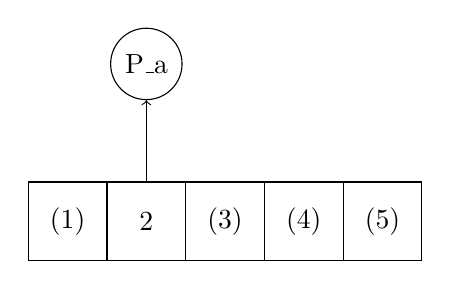
\begin{tikzpicture}
						\node[draw=black, text=black, shape=rectangle, minimum width=1cm, minimum height=1cm] (m_1) at (0,0) (1, 1) {(1)};
						\node[draw=black, text=black, shape=rectangle, minimum width=1cm, minimum height=1cm] (m_2) at (1,0) {2};
						\node[draw=black, text=black, shape=rectangle, minimum width=1cm, minimum height=1cm] (m_3) at (2,0) {(3)};
						\node[draw=black, text=black, shape=rectangle, minimum width=1cm, minimum height=1cm] (m_4) at (3,0) {(4)};
						\node[draw=black, text=black, shape=rectangle, minimum width=1cm, minimum height=1cm] (m_5) at (4,0) {(5)};

						\node[draw=black, text=black, shape=circle, minimum size=0.5cm] (p_a) at (1,2) {P\_a};

						\draw[->] (m_2.north) -- (p_a.south);
					\end{tikzpicture}
				\end{center}
				\caption{Ajout du paragraphe A}
			\end{figure}

			Les autres numéros sont représentés mais mis entre parenthèse car ils n'existent pas dans la Map. Ils sont uniquement là pour nous aider à bien visualiser ce dont on parle. Si nous décidons maintenant d'ajouter un second paragraphe alors celui-ci sera à la position 3.

			\begin{figure}[H]
				\begin{center}
					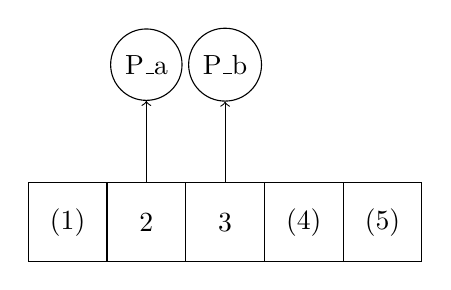
\begin{tikzpicture}
						\node[draw=black, text=black, shape=rectangle, minimum width=1cm, minimum height=1cm] (m_1) at (0,0) (1, 1) {(1)};
						\node[draw=black, text=black, shape=rectangle, minimum width=1cm, minimum height=1cm] (m_2) at (1,0) {2};
						\node[draw=black, text=black, shape=rectangle, minimum width=1cm, minimum height=1cm] (m_3) at (2,0) {3};
						\node[draw=black, text=black, shape=rectangle, minimum width=1cm, minimum height=1cm] (m_4) at (3,0) {(4)};
						\node[draw=black, text=black, shape=rectangle, minimum width=1cm, minimum height=1cm] (m_5) at (4,0) {(5)};

						\node[draw=black, text=black, shape=circle, minimum size=0.5cm] (p_a) at (1,2) {P\_a};
						\node[draw=black, text=black, shape=circle, minimum size=0.5cm] (p_b) at (2,2) {P\_b};

						\draw[->] (m_2.north) -- (p_a.south);
						\draw[->] (m_3.north) -- (p_b.south);
					\end{tikzpicture}
				\end{center}
				\caption{Ajout du paragraphe B}
			\end{figure}

			Maintenant, supposons que nous souhaitons que notre paragraphe A soit le premier noeud du livre, alors il suffira de l'ajouter dans la map l'indice 1 et de supprimer la clé 2 de notre Map.

			\begin{figure}[H]
				\begin{center}
					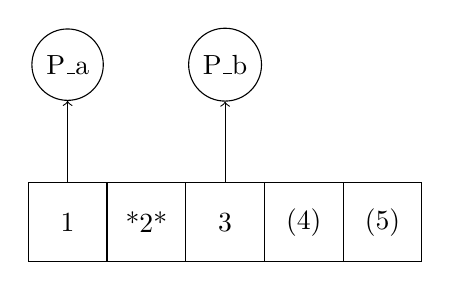
\begin{tikzpicture}
						\node[draw=black, text=black, shape=rectangle, minimum width=1cm, minimum height=1cm] (m_1) at (0,0) {1};
						\node[draw=black, text=black, shape=rectangle, minimum width=1cm, minimum height=1cm] (m_2) at (1,0) {*2*};
						\node[draw=black, text=black, shape=rectangle, minimum width=1cm, minimum height=1cm] (m_3) at (2,0) {3};
						\node[draw=black, text=black, shape=rectangle, minimum width=1cm, minimum height=1cm] (m_4) at (3,0) {(4)};
						\node[draw=black, text=black, shape=rectangle, minimum width=1cm, minimum height=1cm] (m_5) at (4,0) {(5)};

						\node[draw=black, text=black, shape=circle, minimum size=0.5cm] (p_a) at (0,2) {P\_a};
						\node[draw=black, text=black, shape=circle, minimum size=0.5cm] (p_b) at (2,2) {P\_b};

						\draw[->] (m_1.north) -- (p_a.south);
						\draw[->] (m_3.north) -- (p_b.south);
					\end{tikzpicture}
				\end{center}
				\caption{Le paragraphe A devient le noeud de départ}
			\end{figure}

			Dès lors, une case vide se retrouve disponible (symbolisé par des **). Ainsi, si l'on souhaite ajouter un noeud, il faudra d'abord compler ce vide. Le prochain paragraphe, le C donc, aura pour numéro le 2.

			\begin{figure}[H]
				\begin{center}
					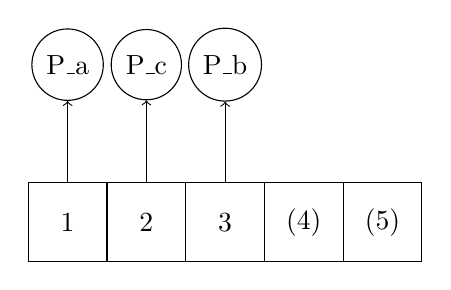
\begin{tikzpicture}
						\node[draw=black, text=black, shape=rectangle, minimum width=1cm, minimum height=1cm] (m_1) at (0,0) {1};
						\node[draw=black, text=black, shape=rectangle, minimum width=1cm, minimum height=1cm] (m_2) at (1,0) {2};
						\node[draw=black, text=black, shape=rectangle, minimum width=1cm, minimum height=1cm] (m_3) at (2,0) {3};
						\node[draw=black, text=black, shape=rectangle, minimum width=1cm, minimum height=1cm] (m_4) at (3,0) {(4)};
						\node[draw=black, text=black, shape=rectangle, minimum width=1cm, minimum height=1cm] (m_5) at (4,0) {(5)};

						\node[draw=black, text=black, shape=circle, minimum size=0.5cm] (p_a) at (0,2) {P\_a};
						\node[draw=black, text=black, shape=circle, minimum size=0.5cm] (p_b) at (2,2) {P\_b};
						\node[draw=black, text=black, shape=circle, minimum size=0.5cm] (p_c) at (1,2) {P\_c};

						\draw[->] (m_1.north) -- (p_a.south);
						\draw[->] (m_2.north) -- (p_c.south);
						\draw[->] (m_3.north) -- (p_b.south);
					\end{tikzpicture}
				\end{center}
				\caption{Ajout du paragraphe C}
			\end{figure}

			Enfin, notre application peut recommencer à ajouter des noeuds à la "fin" de notre Map.

			\begin{figure}[H]
				\begin{center}
					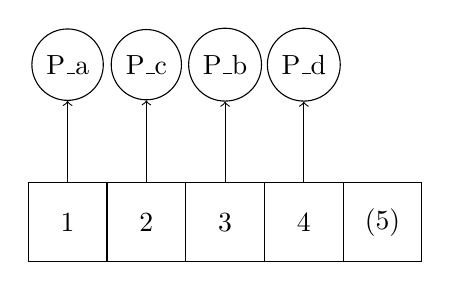
\begin{tikzpicture}
						\node[draw=black, text=black, shape=rectangle, minimum width=1cm, minimum height=1cm] (m_1) at (0,0) {1};
						\node[draw=black, text=black, shape=rectangle, minimum width=1cm, minimum height=1cm] (m_2) at (1,0) {2};
						\node[draw=black, text=black, shape=rectangle, minimum width=1cm, minimum height=1cm] (m_3) at (2,0) {3};
						\node[draw=black, text=black, shape=rectangle, minimum width=1cm, minimum height=1cm] (m_4) at (3,0) {4};
						\node[draw=black, text=black, shape=rectangle, minimum width=1cm, minimum height=1cm] (m_5) at (4,0) {(5)};

						\node[draw=black, text=black, shape=circle, minimum size=0.5cm] (p_a) at (0,2) {P\_a};
						\node[draw=black, text=black, shape=circle, minimum size=0.5cm] (p_b) at (2,2) {P\_b};
						\node[draw=black, text=black, shape=circle, minimum size=0.5cm] (p_c) at (1,2) {P\_c};
						\node[draw=black, text=black, shape=circle, minimum size=0.5cm] (p_d) at (3,2) {P\_d};

						\draw[->] (m_1.north) -- (p_a.south);
						\draw[->] (m_2.north) -- (p_c.south);
						\draw[->] (m_3.north) -- (p_b.south);
						\draw[->] (m_4.north) -- (p_d.south);
					\end{tikzpicture}
				\end{center}
				\caption{Ajout du paragraphe D}
			\end{figure}

			Voici quelques précisions supplémentaires :

			\begin{itemize}
				\item{Le principe d'indice manquant fonctionne également pour la suppression d'un noeud}
				\item{Afin de gagner en performance dans la recherche d'un numéro d'un noeud (pour savoir quel numéro sera manquant par exemple), une autre HashMap est mis à jour en même temps que celle des noeuds. Il s'agit de nodeInv. Cette map n'est rien de plus qu'une sorte de mirroir pour celle des noeuds, on lui passe un noeud en clé et on obtient son indice. Il est donc extrêmement important que les deux maps soient parfaitement identique pour éviter tous bugs.}
				\item{\label{subsec:noeud_delete_missing_index}Pour déterminer l'indice d'un noeud, nous nous basons sur la taille de la Map. Cela pose problème dans un cas particulié. En effet, si nous supprimons un paragraphe au milieu de la map, le noeud à l'indice 3, par exemple, alors cet indice sera libre. Si nous sauvegardons et décidons d'ouvrir de nouveau le fichier, alors nous n'aurons plus cette liste. Il faudrait que nous parcourions la Map pour trouver les indices manquant à la lecture du livre, cependant, comme évoqué un peu partout dans ce rapport, nous avons manqué de temps, d'autant plus que nous pensé à ce détails quelques jours avant de rendre le rapport.}
			\end{itemize}

			De ce fait, voici l'algorithme que nous avons mis en place pour l'ajout d'un noeud.

			\begin{algorithm}[H]
				\DontPrintSemicolon
				\KwIn{le noeud à ajouter : node}
				\KwData{
					nodes : Map<Integer, AbstractBookNode> liste des noeuds\;
					nodesInv : Map<AbstractBookNode, Integer> liste inversée des noeuds\;
					missingIndexes : List<Integer> liste des indices libres\;
				}

				\uIf{node in nodes}{
					\Return{}
				}

				\uIf{missingIndexes.length == 0}{
					offset: int\;
					offset $\gets$ (1 in nodes) ? 1 : 2\;
					nodes[nodes.length + offset] $\gets$ node\;
					nodesInv[node] $\gets$ nodesInv.length + offset\;
				}
				\uElse{
					nodes[missingIndexes[0]] $\gets$ node\;
					nodesInv[node] $\gets$ missingIndexes[0]\;
					missingIndexes.remove(0)\;
				}

				notifyNodeAdded(node)
				\caption{Ajout d'un noeud}
			\end{algorithm}

			La variable offset correspond au décalage à ajouter pour placer le noeud. Comme on commence à 2 un décalage de 2 est nécessaire. Supposons que le premier noeud est renseigné et qu'il est le seul du tableau. Ajouter un noeud le placerait à la position 2 + tailleDuTableau soit 2 + 1 c'est à dire 3. On a un décalage de un. De ce fait, on doit faire un décalage de 1 uniquement si le premier noeud est renseigné.

			Voyons maintenant celui mis en place pour le changement du premier noeud.

			\begin{algorithm}[H]
				\DontPrintSemicolon
				\KwIn{le noeud à ajouter : node}
				\KwData{
					nodes : Map<Integer, AbstractBookNode> liste des noeuds\;
					nodesInv : Map<AbstractBookNode, Integer> liste inversée des noeuds\;
					missingIndexes : List<Integer> liste des indices libres\;
				}

				\uIf{not (node in nodes)}{
					addNode(node)
				}
				\;
				updateDestinations(1, -1)\;
				\;
				indexOfNode: int\;
				indexOfNode $\gets$ nodesInv[node]\;
				\;
				oldNode: AbstractBookNode\;
				oldNode $\gets$ nodes[1]\;
				\;
				updateDestinations(indexOfNode, 1)\;
				\;
				nodes[1] $\gets$ node\;
				nodesInv[node] $\gets$ 1\;
				\;
				\uIf{oldNode != null}{
					nodes[indexOfNode] $\gets$ oldNode\;
					nodesInv[oldNode] $\gets$ indexOfNode\;

					updateDestinations(-1, indexOfNode)\;
				}
				\uElse {
					missingIndexes.add(indexOfNode)\;
					nodes.remove(indexOfNode)\;
				}

				\caption{Changement du premier noeud}
			\end{algorithm}

			\textit{updateDestinations permet de changer les numéro de destination des BookNodeLink d'un ancien numéro, vers un nouveau}

		\subsection{Le pattern observer et la classe Book}
			\label{subsec:pattern_observer}

			Le pattern observer est essentiel pour la mise en place du pattern MVC. Nous avons décidé de procéder de la manière suivante :

			\begin{figure}[H]
				\centering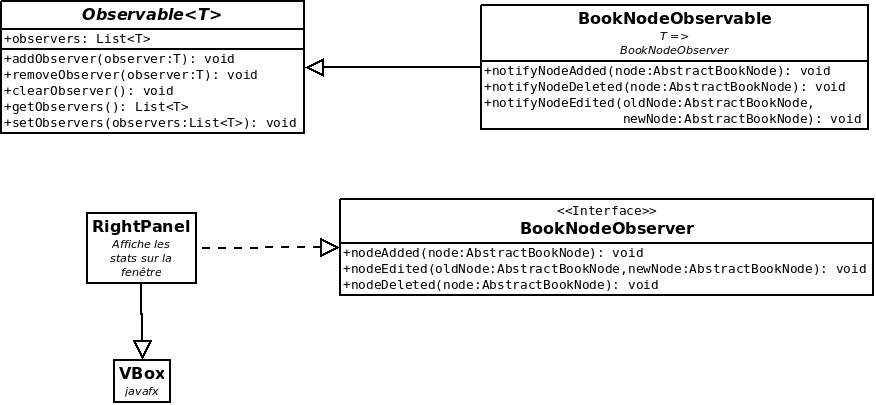
\includegraphics[width=0.8\textwidth, keepaspectratio]{img/observer.png}
				\caption{UML d'exmple sur le pattern observer}
			\end{figure}

			Comme on peut le voir, une classe mère \textbf{Observable<T>} détient une List<T> d'observers. Une méthode d'ajout, et de suppression permettent de modifier cette liste. Dès lors que l'on souhaite ajouter un nouveau type d'observer, on doit commencer par créer une nouvelle Interface avec les méthodes que l'on souhaite fournir, dans notre exemple il s'agit de nodeAdded, nodeEdited, nodeDeleted. Une fois cette interface faite, on doit alors faire une nouvelle classe Observable, BookNodeObservable dans notre cas, qui hérite de Observable<T>, T étant l'observer que l'on souhaite utiliser, donc BookNodeObserver. Ainsi, chaque Observable que l'on fera ne sera qu'une définition des méthodes pour notifier qu'un évènement s'est produit.

			Le choix à été fait de séparer les différentes parties (noeuds, liens, items, ...) du livre en différents observers afin de ne pas surcharger le nombre de méthodes à redéfinir dans les classes Observer, et donc de n'observer que ce dont on a besoin. De ce fait, tous les observers concernant le livre sont sont disponibles sauf celui pour notifier d'un changement concernant le premier noeud.

	\section{Lecture et écriture d'un livre}\label{Json}

		L'objectif de l'application étant de concevoir un éditeur, il était important de permettre la sauvegarde et la lecture du livre que l'on édite. Le choix du format JSON est rapidement survenue. Premièrement car un fichier d'exemple qui nous a été fournis était sous ce format mais aussi car il s'agit d'une structure simple et très facile à lire. Nous avon alors utilisé GSON, une librairie, conçue par Google, extrêmement simple. Elle permet de retranscrire sous forme d'objet Java un fichier JSON structuré, c'est à dire où l'on distingue très clairement des objets qui se répète.

		Afin de lire un fichier JSON, avec cette librairie, il suffit de concevoir des objets Java avec les même attributs que ceux du fichier à lire ou à écrire. Voici un exemple très court de ce à quoi nos fichiers ressembles :

		\subsection{La structure du JSON}

			\begin{lstlisting}[gobble=12, language=json, caption=Exemple de livre très simple, label=lst:exemple_livre]
			{
				"prelude": "Vous êtes l'enseignant qui note notre projet",
				"setup": {
					"skills": [],
					"items": [],
					"characters": [],
					"character_creation": []
				},
				"sections": {
					"1" : {
						"text": "Vous être en train d'étudier notre projet",
						"choices": [
							{
								"text": "Mettre une bonne note",
								"section": 3
							},
							{
								"text": "Mettre une mauvaise note",
								"section": 2
							}
						]
					},
					"2": {
						"text": "Les étudiants du projet sont tristes",
						"end_type": "FAILURE"
					},
					"3": {
						"text": "Les étudiants sont satisfait de leur travail",
						"end_type": "VICTORY"
					}
				}
			}
			\end{lstlisting}

		On retrouve plusieurs éléments différents. On remarque par exemple un attribut "prelude", ainsi que deux grosses parties, "setup" et "sections". Dans la suite, nous détaillerons uniquement les attributs les plus frequemment présents.

		\subsubsection{Setup}

			Commençons par détailler "setup". Ce passage contient toutes les informations générales à notre livre. On y retrouve la liste des compétences ("skills"), la liste des items ("items") et la liste des personnages ("characters"). "character\_creation", lui, détaille toutes les étapes lors de la conception du personnage qui intervient au tout début. Celle-ci permet de sélectionner des skills et items de départ.

			Pour le moment les compétences sont uniquement composé d'un id et d'un nom. Dans une future \maj{} il serait intéressant d'ajouter des propriétés pour connaitre la force ajouté dans un combat, la quantité de soins à rendre par noeuds, par exemple.

			\begin{lstlisting}[gobble=12, language=json, caption=Exemple de compétence]
			{
				"id": "sixth_sense",
				"name": "Sixième sens"
			}
			\end{lstlisting}

			Les items peuvent être de différents types : KEY\_ITEM, WEAPON, DEFENSE, MONEY, HEALING. On retrouve pour tous les items un id et un nom ("name"). Pour certains types, des attributs supplémentaires sont présent. Par exemple, un attribut "durability" peut être présent. Il permet de déterminer le nombre d'utilisation maximum d'un item. Un item de type HEALING possède un nombre de pv à rendre ("hp") tandis que ceux type WEAPON possède un montant de dégats ("damage") par exemple.

			\begin{lstlisting}[gobble=12, language=json, caption=Exemple d'items]
			{
				"id": "backpack",
				"name": "Backpack",
				"item_type": "KEY_ITEM"
			},
			{
				"id": "healing_potion_4",
				"name": "Potion de soins (4HP)",
				"hp": 4,
				"durability": 1,
				"item_type": "HEALING"
			}
			\end{lstlisting}

			Concernant les personnages on y retrouve un id, un nom ("name"), un nombre de pv maximum ("hp"), un boolean pour indiquer s'il a beaucoup de chance que ses coups fassent le double des dégats ("double\_damage"), ainsi que "combat\_skill" qui représente le montant de ses dégats.

			\begin{lstlisting}[gobble=12, language=json, caption=Exemple de personnage]
			{
				"id": "zombie_captain",
				"name": "Zombie Captain",
				"hp": 15,
				"double_damage": true,
				"combat_skill": 2
			}
			\end{lstlisting}

			Les character character\_creation peuvent être de simple texte ou de type "ITEM" ou "SKILL". On y retrouve les différents skills ou items que l'on peut prendre pour débuter notre aventure ainsi que le nombre que l'on doit en choisir ("amount\_to\_pick").

			\begin{lstlisting}[gobble=12, language=json, caption=Exemple de character\_creation]
			{
				"text": "Kai Disciplines\n\nOver the centuries, the Kai monks have mastered the skills of the warrior. These skills are known as the Kai Disciplines, [...]",
				"type": "SKILL",
				"skills": [
					"camouflage",
					"hunting",
					"sixth_sense",
					"tracking",
					"healing",
					"weaponskill",
					"mindshield",
					"mindblast",
					"animal_kinship",
					"mind_over_matter"
				],
				"amount_to_pick": 5
			}
			\end{lstlisting}

		\subsubsection{Sections}

			La partie "sections" est une map qui représente le numéro d'un paragraphe ainsi que le paragraphe associé. Il existe différents types de paragraphes, à choix, à choix aléatoire, avec des combats, terminaux. Tous possède un texte. Les noeuds terminaux possèdent un type de fin ("end\_type") afin savoir si l'on a gagné ou pas (cf : Listing \ref{lst:exemple_livre}). Les noeuds aléatoires eux, possède un attribut "is\_random\_pick" qui vaut true. Pour tous les autres types de noeuds, on retrouve parmis les attributs les plus importants une liste d'items qu'il est possible de prendre, un montant d'item maximum qui peut être pris ("amount\_to\_pick"), des items disponibles à l'achat ("shop").

			\begin{lstlisting}[gobble=12, language=json, caption=Exemple de paragraphe]
			{
				"text": "The back door opens [...]",
				"items": [
					{
						"id": "gold",
						"amount": 5
					},
					{
						"id": "dagger"
					},
					{
						"id": "seal_hammerdal"
					}
				],
				"amount_to_pick": 2
				"choices": [
					{
						"text": "Return to the tavern.",
						"section": "177"
					},
					{
						"text": "Study the tomb.",
						"section": "24"
					}
				]
			}
			\end{lstlisting}

			Certains paragraphes peuvent contenir un attribut "combat". Dès lors on peut connaitre le choix en cas de victoire ("win"), de défaite ("loose") ou d'évasion ("evasion). Si l'évasion est possible seulement à partir d'un certains nombre de tour on retrouve alors un attribut nommé "evasion\_round". Pour finir, un attribut "enemies" permet de connaitre les personnages que l'on combat.

			\begin{lstlisting}[gobble=12, language=json, caption=Exemple de paragraphe avec des combats]
			{
				"text": "The dead zombies lie [...]",
				"combat": {
					"win": {
						"text": "If you win the combat.",
						"section": "309"
					},
					"enemies": [
						"zombie_captain"
					]
				}
			}
			\end{lstlisting}

			Pour représenter un lien vers un autre paragraphe on retrouve une liste de choix ("choices"). Ils possèdent également un texte qui correspond à l'intititulé du choix, le numéro du paragraphe suivant ("section"), un nombre d'hp à retirer, un nombre d'argent à ajouter ainsi qu'un liste de prérequis ("requirements"). Comme pour les BookNodeLink, il s'agit d'un tableau à deux dimensions. Le premier représente une liste de condition en OU et le second une liste de condition en ET. Enfin, pour les noeuds aléatoire, un poid est également présent ("weight").

			\begin{lstlisting}[gobble=12, language=json, caption=Exemple de choix]
			{
				"text": "If you have the Kai Discipline of Tracking.",
				"section": "182",
				"hp": -5,
				"requirements":  [
					[
						{
							"id": "tracking",
							"type": "SKILL"
						}
					]
				]
			}
			\end{lstlisting}

		\subsection{La lecture et l'écriture}
			\label{subsec:lecture_ecriture_fichier}

			Du fait que la structure en Json n'est pas identique à celle détaillé dans \nameref{sec:representation_livre} (page \pageref{sec:representation_livre}), nous avons fait des classes intermédiaires pour permettre cette lecture. Celles-ci sont disponibles dans le package \textit{magic\_book/core/file/json} et ne contiennent rien de plus que des getter et setter. Aussi, afin de permettre une convertion entre les classes faites pour représenter un fichier json et celles faites pour être utilisées par l'application, une interface \textit{JsonExportable} existe. Celle ci permet de redéfinir 2 méthodes. L'une renvoyant la classe JSON associé à notre classe actuelle, l'autre permettant à partir d'une classe JSON d'obtenir la classe Java correspondante.

			\begin{figure}[H]
				\centering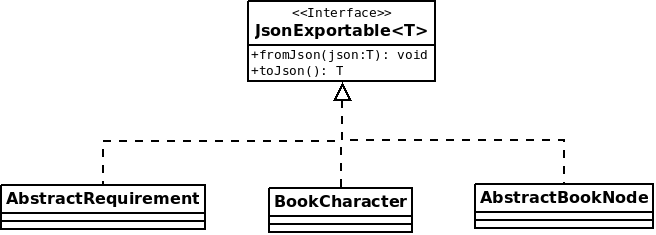
\includegraphics[width=0.66\textwidth, keepaspectratio]{img/json_exportable.png}
				\caption{L'interface JsonExportable et quelques classes qui l'implémentent}
			\end{figure}

			Enfin, les classes BookReader et BookWritter permettent de récupérer toutes les classes JSON intermédiaires pour les regrouper dans le BookJson qui correspond à la structure complète de notre livre. Ces classes sont également une couche d'abstraction à GSON car c'est elles qui se chargent d'écrire le JSON correspondant dans un flux.

			Pour résumer, on peut schématiser ces échanges de telle sorte :

			\begin{figure}[H]
				\begin{center}
					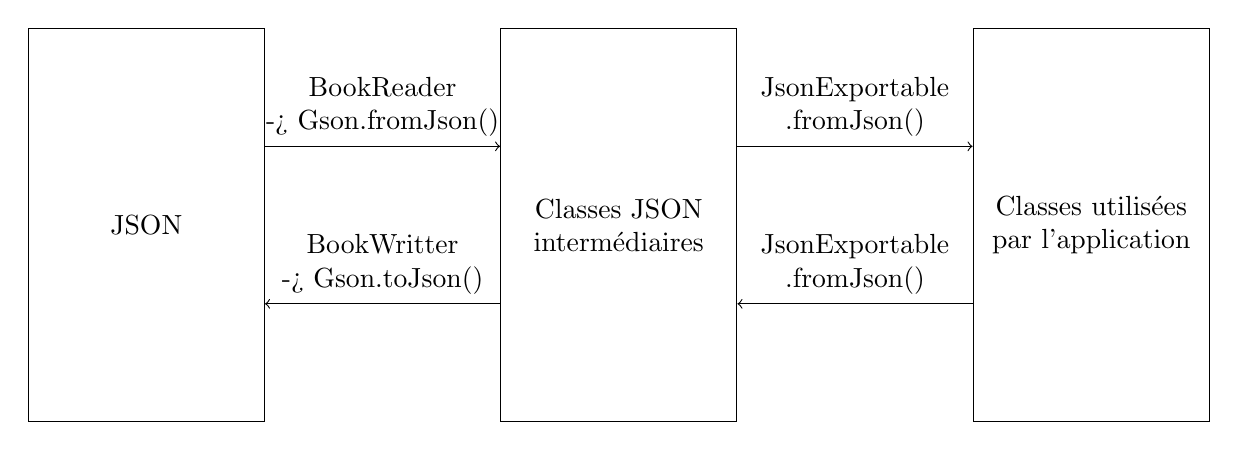
\begin{tikzpicture}
						\node[draw=black, text=black, shape=rectangle, minimum width=3cm, minimum height=5cm] (json) at (0,0) {JSON};
						\node[draw=black, text=black, shape=rectangle, minimum width=3cm, minimum height=5cm, align=center] (json_class) at (6,0) {Classes JSON\\ intermédiaires};
						\node[draw=black, text=black, shape=rectangle, minimum width=3cm, minimum height=5cm, align=center] (class) at (12,0) {Classes utilisées\\ par l'application};

						\draw[->] ([yshift=1cm]json.east) -- node[above, align=center] {BookReader\\ \fontsize{10}{12}\selectfont-> Gson.fromJson()}([yshift=1cm]json_class.west);
						\draw[->] ([yshift=-1cm]json_class.west) -- node[above, align=center] {BookWritter\\ \fontsize{10}{12}\selectfont-> Gson.toJson()}([yshift=-1cm]json.east);

						\draw[->] ([yshift=1cm]json_class.east) -- node[above, align=center] {JsonExportable\\.fromJson()}([yshift=1cm]class.west);
						\draw[->] ([yshift=-1cm]class.west) -- node[above, align=center] {JsonExportable\\.fromJson()}([yshift=-1cm]json_class.east);
					\end{tikzpicture}
				\end{center}
				\caption{Échanges pour la lecture / écriture}
			\end{figure}

	\section{Edition graphique d'un livre}
		Afin d'éditer un livre, nous avons différents boutons permettant de changer de mode. Chaque mode permet d'ajouter, de supprimer, de sélectionner, un noeud ou un lien. Ces modes sont gérer à l'aide de la MainWindows qui est une fenêtre qui affiche tout les différents panel. Il existe trois grand panel  (Voir\ref{fig:MainWindows}) comportant eux même d'autre petit panel. Le premier panel se nomme le \textbf{LeftPane}. Il se situe à gauche et est composé des boutons de mode, d'une liste d'item existant ainsi que d'une liste de personnage existant. Le deuxième panel s'appel le \textbf{GraphPane}. Il est au centre et permet d'ajouter les noeuds ainsi que les liens entre les noeuds. Il contient également le prélude. Le troisième panel se nomme le \textbf{RightPane}. Il permet d'afficher les statistiques du livre comme par exemple, le nombre de noeud et l'estimation de la difficulté du livre.\\
		\begin{figure}[H]
			\centering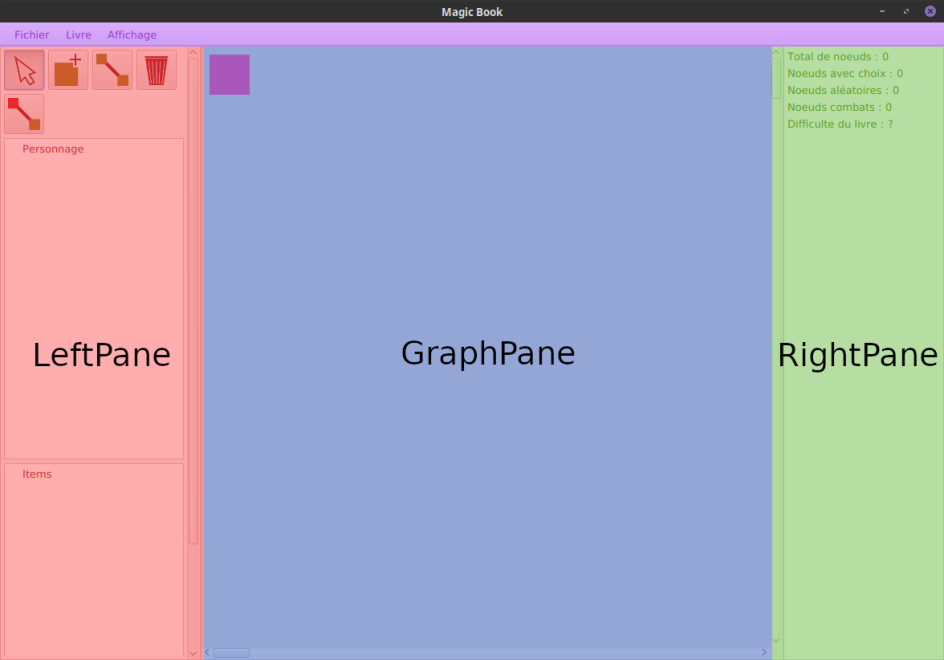
\includegraphics[width=0.50\textwidth]{img/mainwindow.png}
			\caption{MainWindows}
			\label{fig:MainWindows}
		\end{figure}

		\subsection{MainWindows}
			La MainWindows, comme mentionné précédement, contient toute la fenêtre. Elle contient également un Menu permettant de réaliser plusieurs actions.\\
			Premièrement, dans le menu nommé \textbf{Fichier}, l'utilisateur peut alors ouvrir un nouveau livre vide en cliquant sur \textbf{Nouveau}. Un nouveau livre est alors ouvert en mettant tout les panel (LeftPane, GraphPane, RightPane) à jour, permettant ainsi de remmettre tout à zéro. Ce menu comporte aussi un MenuItem nommé \textbf{Ouvrir}, permettant ainsi d'ouvrir un fichier Json ou txt. Si ce fichier n'est pas bien indenté, il manque une virgule ou une accolade ou autre ne permettant pas la lecture du fichier en Json (Voir \ref{Json}), un message d'erreur apparait. Si le fichier n'est pas bien fait, ne permettant pas l'ouverture de ce fichier, une classe nommé \textbf{BookValidator} devait "valider" le livre. Par manque de temps, cette classe n'est pas fonctionnelle. Si le fichier est bien indenté et peut s'ouvrir, le livre est changé en mettant tout les panel à jour. Il peut aussi enregistrer ou enregistrer-sous le livre en faisant appel au FileChooser et au File.\\
			Deuxièmement, dans le menu nommé \textbf{Livre}, l'utilisateur peut \textbf{Jouer} ou \textbf{Estimer la difficulté}. Ces deux MenuItem utilisent toutes les deux la classe Jeu, décrit un peu plus loin \ref{Jeu}. Un autre MenuItem est aussi présent, permettant de \textbf{Générer le livre en txt}. Cela permet à l'utilisateur de pouvoir avoir un livre propre contenant les paragraphes et le choix de chaque paragraphes.\\
			Troisièmement, dans le menu nommé \textbf{Affichage}, l'utilisateur peut afficher ou non, le LeftPane et/ou le RightPane. Cela permet notament à l'utilisateur de mieux voir la partie édition. Mais était surtout réalisé pour un meilleur affichage en vidéo projecteur de notre projet.\\


		\subsection{LeftPane}
			Ce panel contient tout d'abord des ToggleButton permettant de sélectionner un mode parmis cinq modes : \textbf{SELECT, ADD NODE, ADD NODE LINK, DELETE, FIRST NODE}. Chacun de ces mode fait appel à une méthode permettant de créer le bouton. Cette méthode prend en paramètre une image et un des modes de la classe Mode.\\
			Ensuite, un TreeItem contenant des BookCharacter est créer permettant de lister tout les personnages créé à l'aide de TreeView. Le même procédé est réalisé pour les items.\\
			Puis, pour permettre à l'utilisateur de créer des items et des personnages, un ContextMenu est ajouter au TreeView des items, puis au TreeView des personnages. Une action est implémenté pour chaque choix de ces ContextMenu: Ajout, Modification, Suppression. Vous trouverez ci dessous, un exemple pour les personnages.

			\begin{lstlisting}[language=java]
				TreeItem<BookCharacter> rootPerso = new TreeItem<> (new BookCharacter("0", "Personnage", 0, 0, null, null, 0));
				rootPerso.setExpanded(true);
				treeViewPerso = new TreeView<> (rootPerso);

				ContextMenu contextMenuPerso = new ContextMenu();
				MenuItem menuPersoAdd = new MenuItem("Ajouter un Personnage");
				MenuItem menuPersoUpdate = new MenuItem("Modifier un Personnage");
				MenuItem menuPersoDel = new MenuItem("Supprimer un Personnage");
			\end{lstlisting}

			Si le choix d'ajout est cliqué, une boite de dialog apparait appelant CharacterDialog qui elle même appel CharacterComponent pour la création d'un personnage ou ItemDialog pour la création d'un item.\\
			Pour ce dernier, l'ItemDialog à une ChoiceBox permettant de choisir si l'item créer est une arme, un item de soin, de défense ou un simple item. Le BookItem est créer en fonction du type d'item.\\
			\begin{centering}
			\begin{figure}[H]
				\begin{subfigure}[b]{0.37\textwidth}
					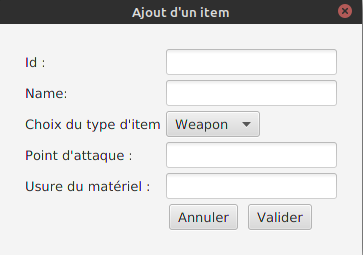
\includegraphics[width=\textwidth, keepaspectratio]{img/item.png}
				\end{subfigure}
				\begin{subfigure}[b]{0.3\textwidth}
					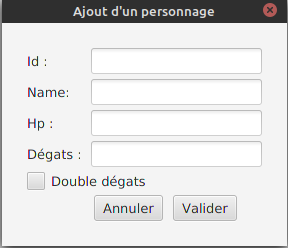
\includegraphics[width=\textwidth, keepaspectratio]{img/personnage.png}
				\end{subfigure}
			\end{figure}
		\end{centering}

		\subsection{GraphPane}

			Le prélude est déjà situé en haut à gauche du GraphPane. Ce prélude, comme les noeuds, est représenté par un carré. Il contient un PréludeFx faisant le lien entre le noeud du prélude et le Rectangle le contenant. Ce prélude contient trois Tab. La première Tab contient le texte du prélude. La deuxième contient la création du personnage. Et la troisième la création du personnage principal.\\
			La deuxième partie du TabPane contient un Accordion. Cette accordion est affiché grâce au bouton \textbf{Ajouter}. Chaque accordion est composé d'un CharacterCreationComponent comprenant un Texte, une CheckBox (Texte, Item), et d'un bouton \textbf{Supprimer cette partie}.\\


			La checkBox n'affiche que \textbf{Texte} si aucun item n'est disponible. Mais si un item est créé, l'utilisateur peu alors ajouter un ItemListComponent en sélectionnant \textbf{Item} dans la CheckBox. Cette classe est affiché sur tout les noeuds, permettant d'ajouter des items ainsi que la quantité disponible de chaque item, qui ici, sera disponible en début de partie. L'item ajouté peut être supprimé grâce à un clic droit de la souris.\\



			La troisième partie du TabPane permet quant a elle, de créer le personnage principal grâce au CharacterComponent. Cette classe permet de créer un personnage. Mais si la valeur boolean de mainCharacter est true, les TextField pour le nombre d'item maximum ainsi que la quantité d'argent est ajouté.
			Après validation, le textPrelude (texte du prélude), mainCharacter (personnage principal) et le characterCreations (item et texte à afficher après le prélude) est créer.


			Pour ajouter un noeud, on clique sur le mode \textbf{ADD NODE},puis on clique sur le GraphPane. Une fenêtre de dialog est alors ouverte afin de renseigner le paragraphe à afficher, ainsi qu'une CheckBox permettant de sélectionner le type de noeud. L'affichage change en fonction du type de noeud sélectionner dans cette CheckBox, qui elle, est prédéfini sur \textbf{Basic}.\\

			Si c'est un noeud basic ou aléatoire, les renseignements suivant sont demandé: le texte à afficher, le nombre de points de vie à gagner/perdre, les items disponible, le nombre d'item disponible. Rien ne change sur la structure de la boite de dialog entre ces deux types. Mais au moment de la validation, le type de BookNode créer se fera en fonction de la valeur de la choiceBox : BoockNodeWithChoices, BookNodeWithRandomChoices. Des try/catch sont utilisé afin de changer certaine valeurs de saisie en Integer. Cela permet d'être sûr que ce sont des chiffres. Si la conversion ne peut pas se faire, une boite de dialog affichant l'erreur apparait, notifiant ainsi où l'erreur se situe.\\

			Si c'est un noeud de combat...... JUJU  :p\\


			Si c'est un noeud terminal, une ChoiceBox est juste rajouté afin de savoir si c'est un noeud gagnant ou perdant. Lors de la validation, un BookNodeTerminal est créer avec comme valeur un BookNodeStatus défini en fonction de la ChoiceBox.\\

			Dès qu'un noeud est validé, un NodeFx est créer. Il contient alors le noeud créer et affiche un Rectangle là où la souris a été cliqué dans le graphPane, à la création du noeud. La couleur du carré change en fonction du type de noeud. Un RectangleFX est donc mis en place permettant d'envoyé une notification si jamais la souris passe dessus (opacité du Rectangle qui change), réalise un clique maintenu (déplacement du rectangle en fonction de la souris), réalise un clique simple. Pour ce dernier, cela envoie une notification à l'observable permettant de prévenir l'observeur qu'on a cliquer dessus. Cela sert si un double clique est produit (permet de procédé à une modification si le mode activé est \textbf{SELECT}, a une suppression si c'est le mode \textbf{DELETE} qui est activé ou encore a une création de lien entre le prélude et le noeud sélectionné si le mode \textbf{FIRST NODE} est activé) ou si un deux cliques espacé sont réalisé (permet de procédé à la création d'un lien si le mode \textbf{ADD NODE LINK} est sélectionné).\\

			Une fois un ou plusieurs noeud créer, un lien peut être donc être effectué. Le lien peut être fait sur le même noeud, si une boucle est voulu. Mais il peut aussi être réalisé entre deux noeuds. Pour ce faire, le mode \textbf{ADD NODE LINK} doit être activé. Le premier clique permet de sauvegarder le noeud de départ. Le deuxième permet d'avoir le noeud de destination. Une fois les deux cliques détecté, une fenêtre de dialog apparait. Il y a trois affichage différent.\\
			L'affiche ce fait en fonction du premier noeud. Tout d'abord, l'affichage commun entre ces noeuds est un simple texte, deux TextField ainsi qu'un CheckBox. Les TextField permettent d'ajouter un gain ou une perte de vie/d'argent. La CheckBox, quant a elle, permet d'aller vers ce choix obligatoirement ou non.\\
			Si le premier noeud est un noeud de combat, une ChoiceBox apparait alors permettant de choisir si c'est un lien gagnant, perdant ou un lien d'évasion. Cette liste de choix est créer si le permier noeud à encore des choix de libre. S'il n'a plus de choix libre, une boite d'alerte s'affiche en prévenant qu'il n'y a plus aucun lien disponible.\\

			Si le permier noeud est de type aléatoire, le joueur doit alors renseigner la chance sur chaque lien.\\

			Le lien est repésenté par une ligne entre le noeuds de départ et d'arrivé. Pour les différencier, un cercle est créer et est affiché au noeud de destination. Tout cela est géré par NodeLinkFx qui a aussi un observeur permettant d'envoyé une notification si jamais la ligne ou le cercle enregistre un événement du style pressed. Cela permet de savoir si le lien a été double cliqué pour réaliser une modification.\\

		\subsection{RightPane}

		Ce panel contient tout ce qui représente les statistiques. Dès qu'un noeud est ajouté ou supprimé, une méthode de la class \textit{RightPane} est utilisé afin de mettre à jour le nombre de noeuds existant. Pour la difficulté du livre, elle est mise à jours dès que \textbf{Estimé la difficulté du livre} est sélectionné.\\
		Si un nouveau livre est chargé, tout ces statistiques ce remmettent à zéro.



	\section{Rendre le livre jouable et estimer sa difficulté}\label{Jeu}
		\subsection{Jeu}
		Une classe à été créer se nommant \textbf{Jeu}, permettant de gérer les méthodes de jeu communes entre le \textit{Player} et les \textit{Fourmis}.\\
		Un construteur est d'abord appelé, à partir de la MainWindows, afin d'envoyer le livre contenant toutes les informations. Puis, en fonction du mode sélectionner (\textbf{Générer la difficulté} ou \textbf{jouer}), la méthode correspondante au player est appelé.\\
		Une fois dans la méthode choisis, le livre est alors copié afin de ne pas le modifier par erreur pendant le jeu. Un BookState, qui correspond à la sauvegarde de la partie, est alors créé. Si le prélude contient un personnage principal, alors celui ci est enregistré dans la sauvegarde de la partie (le BookState). Dans le cas contraire, un autre personnage principal est créer afin de pouvoir jouer au jeu.\\
		\begin{lstlisting}[language=java]
			BookState newState = new BookState()
			if(this.book.getMainCharacter() == null){
				//Création d'un BookCharacter
			} else {
				BookCharacter bookCharacterMain = this.book.getMainCharacter();
			}
			newState.setBook(this.book);
			for(AbstractCharacterCreation characterCreation : this.book.getCharacterCreations())
				player.execPlayerCreation(book, characterCreation, newState);

			return newState;
		\end{lstlisting}
		Enfin, si des compétences et/ou des items sont disponible au début de la partie, la méthode de création de joueur est appelé en focntion du player actuel. Comme cela, le player choisit parmi une liste de skill et d'items disponible en début de partie afin de les avoir pour commencer le jeu.\\
		Une fois le BookState créer, le personnage principal initialisé et la copie du livre enregistré, le premier noeud est donc chargé. Une méthode est appelé en fonction de son type de noeud. La méthode correspondante au type de noeud s'exécute et renvoie le noeud de destination, en fonction du choix du player et/ou de la mort du player. Durant l'exécution des différentes méthodes et en fonction du player, d'autre méthode externe sont appelé nottament dans la classe Fourmis ou Player.\\
		\begin{lstlisting}[language=java]
			while(!gameFinish){
				if(currentNode instanceof BookNodeCombat){
					//execNodeCombat(bookNodeCombat);
				}
				else if(currentNode instanceof BookNodeWithChoices){
					//execNodeWithChoices(bookNodeWithChoices);
				}
				else if(currentNode instanceof BookNodeWithRandomChoices){
					//execNodeWithRandomChoices(bookNodeWithRandomChoices);
				}
				else if(currentNode instanceof BookNodeTerminal){
					//execNodeTerminal(bookNodeTerminal);
					//Si partie gagné, win = true
				} else {
					//BookNodeTerminal FAILURE
				}
			}
			return win;
		\end{lstlisting}

		Pour chaque type de noeud, sauf pour un noeud terminal, une méthode commune est appelé afin de savoir si le noeud pris en charge fait gagné/perdre de la vie puis regarde si le player est toujours en vie. Si ce dernier n'est plus en vie, un noeud terminal est alors renvoyé en noeud de destination. S'il est encore en vie et que le noeud propose des items, ils sont proposés au player en appelant la méthode correspondante entre Fourmis ou Player. A chaque detination choisi, une autre méthode est appelé afin de regarder si le lien entre le noeud de départ et de destination fait perdre ou gagner de la vie et/ou de l'argent.\\

		\textbf{Si un noeud est de type basic}, il est alors pris en charge dans la méthode \textit{execNodeWithChoices}. Cette dernière renvoi un noeud terminal si aucun choix n'est valide, ce qu'il veut dire, si le player n'a aucun choix ou s'il ne possède pas les items/skill pour aller vers ce choix.\\
		Si le player est encore en vie et si il peut au moins choisir une destination, un choix est demandé parmis toutes les destinations faisant un appel à la méthode en fonction du player. Si le player a les prérequis pour aller vers cette destination, alors le noeud choisi est renvoyé en noeud de destination. Sinon, le player doit faire un autre choix.\\

		\textbf{Si c'est un noeud de type combat}, une vérification est réalisé afin savoir si le noeud contient des ennemis. S'il n'y a pas d'ennemis, le noeud en cas de victoire est envoyé en noeud de destination. Sinon, une liste d'ennemis est créer afin de ne pas modifié la vie des ennemis. Car ces derniers ne sont pas lié au noeud, mais c'est l'ID de l'ennemis qui est lié au noeud permettant de les appelés plusieurs fois dans plusieurs ou dans le même noeud.\\
		Le combat commence alors. Le choix est défini par la méthode du player correspondant. Trois choix sont possible:\\
		\begin{description}
			\item[Attaque :]{un autre choix est demandé permettant de sélectionner l'ennemi à attaquer parmi la liste des ennemis encore en vie. Une fois l'ennemi sélectionné, une méthode attaque est appelé apellant elle même une autre méthode commune entre l'attaque du player et l'attaque d'ennemi. Nommé \textit{getDamageAmount}, elle permet de savoir le nombre de dommage réalisé en fonction des point d'attaque de l'attaquant, de son double dommage décider en random si ce boolean est défini en true, d'un coup critique décider aussi en random, de l'arme de l'attaquant et de l'item de défense de l'attaqué. L'attaquant et l'attaqué est défini en fonction de la permière méthode qui l'appel. Ici c'est la méthode d'attaque du player.}
			Une fois l'attaque effectué, si l'ennemi attaqué est mort, il est supprimer de la liste des ennemis.
			\item[Inventaire :]{si ce choix est fait par le player, la méthode appelé permettant d'utiliser son inventaire est elle même gérer dans la classe Player ou la classe Fourmis. Elle permet alors de choisir une potion, une arme et ou un item de défense.}
			\item[Evasion :]{si le tour avant évasion est inférieur ou égal à 0 et si un noeud de d'évasion existe, le player peut alors s'enfuir. Sinon cela lui passe son tour.}
		\end{description}

		Une fois le tour du joueur fini, vient le tour de l'ennemi. Il appel une méthode envoyant la liste d'ennemis restant. Cette méthode appel \textit{getDamageAmount} permettant aux ennemis d'attaquer un par un.\\

		Une fois le tour du joueur fini, vient le tour de l'ennemi. Il appel une méthode envoyant la liste d'ennemis restant. Cette méthode appel \textit{getDamageAmount} permettant aux ennemis d'attaquer un par un.

		La fin de combat est déterminé si la liste d'ennemis est vide ou si le player n'est plus en vie. Le noeud de destination est alors défini en fonction du résultat en fin de combat.

		\textbf{Si le noeud est de type aléatoire}, la méthode commune est appelé afin de savoir si le player est encore en vie. Puis une autre méthode est appelé afin de déterminer le noeud de destination en fonction des chances attribué à chacun de ces choix.\\

		\textbf{Si le noeud est de type terminal}, la partie est alors terminé et renvoie un bolean sur l'état de la fin de partie.\\

	\subsection{Interface Player / Foumis}
		Une interface \textbf{InterfacePlayerFoumis} à été créer permettant une mise en commun des codes Player et Fourmis. Ces méthodes permettent de faire un choix, prendre les items disponibles, créer un personage lambda, aller dans l'inventaire, choisir son ennemis ou encore combatre. Elles sont appelé au même moment. La méthode sera alors exécuté différément en fonction du player.\\

		\textit{execPlayerCreation} permet de choisir les skill et les items disponible au début de la partie. Ces derniers sont défini lors de la création du prélude. Pour l'ajout des items, la méthode \textit{prendItems} est appelé.\\

		\textit{combatChoice}, prend en paramètre le noeud de Combat et le nombre de tour avant l'évasion ainsi que le BookState, permet de faire un choix lors du tour du player dans un combat. On peut alors choisir d'attaquer, d'aller dans l'inventaire ou alors de s'évader. Si on choisi l'inventaire, on va alors dans une autre méthode appelé useInventaire() qui prend le BookState en paramètre. On peut alors utiliser une potion, prendre un objet de défense ou alors une arme. Si l'on choisis un autre choix, cette objet n'est pas utilisable lors d'un combat (comme par exemple de l'argent). Une fois l'objet pris, on retourne dans les choix du combat. On peut alors, soit retourner dans l'inventaire pour prendre un autre objet, soit attaquer ou s'évader.\\

		\textit{chooseEnnemi} permet de choisir l'ennemi à attaquer parmi la liste de tout les ennemis encore en vie.\\

		\textit{prendItems} permet de prendre un item parmi la liste d'items disponible. Cette liste est pris en paramètre ainsi que la sauvegarde de la partie et le nombre d'item maximum pouvant être pris.\\

		\textit{makeAChoice} permet de faire un choix en fonction des différentes destinations proposé par le noeud.\\

		\textit{useIventaire} permet d'utiliser son inventaire lors d'un noeud de combat. La mise à jour d'un port d'item de défense ou d'arme est alors mis à jour. Si un item de soin est choisi, les points de vie du joueur sont alors actualisé.\\

	\subsection{Player}
		La classe \textbf{Player} permet de jouer au jeu en tant que joueur. Elle permet de faire des choix grâce aux Scanner. Des messages sont aussi affiché afin de guider le joueur dans ses choix.\\
		Notament la méthode \textit{choixYesNo} qui permet de choisir oui ou non et de renvoyer le boolean true ou false. Cette méthode permet, par exemple, de savoir si le player veut supprimer, prendre un item ou un skill.\\
		Pour la méthode commune \textit{prendItems}, cette dernière fait appel à d'autre méthode dans la classe Player. Comme itemAdd() permettant de choisir l'item à ajouter dans l'inventaire. Ou encore itemPlein() qui demande au joueur s'il veut supprimer un item. Si le joueur répond oui, la méthode itemSupp() est appelé afin de choisir l'item à supprimer et à mettre à jour l'inventaire.\\
		Pour la méthode \textit{execPlayerCreation} au moment de l'ajout des skill, le joueur doit confimer ou non s'il veut un skill. Si oui, la méthode skillAdd est appelé jusqu'à ce que le maximum d'item à été pris ou qu'ilne reste plus de skill à prendre.\\

	\subsection{Fourmis}
		La classe \textbf{Fourmis} permet de jouer en tant que joueur fictif. Elle effectue des choix random en fonction des différentes méthodes de l'interface.
		Comme par exemple, pour prendre des items ou des skill, la fourmi en prend autant que possible et en supprime obligatoirement en aléatoire si il n'a plus de place dans l'inventaire. Nous avons décider de réalisé cette méthode comme cela afin de pouvoir aller dans le maximum de noeud s'ilsont des prérequis ou alors avoir le maximum d'items pour les combats.\\
		Pour la méthode \textit{chooseEnnemi}, la fourmi envoyé prend obligatoirement le premier ennemi permettant de tué le maximum d'ennemis en attaquant toujours le même ennemis.\\
		Et enfin, la méthode \textit{combatChoice} permet de choisir entre ATTAQUE, EVASION, INVENTAIRE. Nous avons choisir de faire un random sur les trois choix et non pas sur deux choix même si le tour d'évasion n'est pas disponible afin de passer le tour, comme le joueur, afn d'avoir la même chance lors des combats.\\
